%==================================================================================================
%   LUKES THESIS TEMPLATE 1.2
%   -------------------------
%   This template is based upon the offcial IMM PhD Thesis template, it is enhanced with a number
%   of new features and a number of errors have fixed. This template is intended to be complied to
%   PDF using PDFLATEX and is tested using the MiKTeX 2.9 LaTeX distribution.
%   It is based on the official DTU-IMM Thesis template by Finn Kuno Christensen in 2009.
%   Small bugfixes by Kasper Laursen in 2012 and 2013.
%   Small updates by Finn Kuno Christensen/Henning Christiansen in 2015.
%   -------------------------
%   Last Updated: 2015-01-08
%==================================================================================================
%
%==================================================================================================
% DOCUMENT SETUP
%==================================================================================================
\documentclass[10pt,twoside]{book}							%Official DTU-IMM Thesis document setup
%
%Set to 'print' for printed version, use 'net' for online version
\def\thesisversion{print}
%
%==================================================================================================
% PACKAGES
%==================================================================================================
\usepackage{LukeThesis}										%Import Thesis base style
%input{PhDMacros}											%Thesis specific macros
%
%==================================================================================================
% THESIS PROPERTIES (Modifiy these fields with your details)
%==================================================================================================
\def\thesisauthor{Carsten Nielsen}							%Author
\def\thesistitle{Developing a StarCraft: Brood War Agent}	%Title
\def\thesishandin{30-June}									%Submission date (Day-Month}
\def\thesisdegree{B.Sc}										%Degree ('B.Eng', 'B.Sc.', 'M.Sc.' or 'PhD')
\def\thesisyear{2015}										%Submission year
\def\thesisnumber{????}										%DTU-IMM Serial number (do not include year)
\def\thesisISSN{0000-0000}									%ISSN number
\def\thesiskeywords{AI, Bot, Starcraft, RTS}				%PDF keywords
\derivethesisprops											%Derive dependent properties
%
%==================================================================================================
% SECTION NUMBERING SETUP
%==================================================================================================
\setcounter{tocdepth}{2}									%2 adds sections up to subsections
\setcounter{secnumdepth}{3}									%Subsubsections get a number when this is 3
%
%==================================================================================================
% THESIS STRUCTURE  (Modifiy to include more chapters etc)
%==================================================================================================
\begin{document}
%------------------------
%Pre-frontmatter material
%------------------------
\prefrontmatter
%--------------------
%Frontmatter material
%--------------------
\frontmatter
\pagenumbering{roman}										%Set frontmatter numbering style
\chapter{Abstract}
This thesis follows the development of a StarCraft: Brood War agent, and explores the challenges which real-time strategy game poses artificial intelligence. It presents simple but efficient solutions to the most important problems. The agent is capable of efficient resource gathering, training and building units and expanding to more bases. Troops are grouped, retreating when outnumbered and attacking when not. Using a Protoss rush strategy, the agent performs very well in the Student StarCraft Artificial Intelligence Tournament, netting an 79.23\% win-rate on average across 700+ matches.											%English summary of Thesis
\markboth{}{}												%Set headings (left)(right)
\chapter{Resumé}
\begin{otherlanguage}{danish}

Målet for denne afhandling er at ...

\end{otherlanguage}											%Danish summary of Thesis
\markboth{}{}												%Set headings (left)(right)
\chapter{Preface}
This thesis was prepared at DTU Compute in fulfillment of the requirements for acquiring an B.Sc. in Engineering.

Starcraft is one of the strongest game franchise ever created. Professional players compete in Starcraft 2 tournaments with large price purses. Perhaps less known is that former developers of Othello and chess playing programs have taken on the task to develop AIs for the game. Most developers use the relatively old Starcraft: Brood War as all the necessary infrastructure is readily available: \url{http://code.google.com/p/bwapi/}. Championships for AIs, bots, are arranged yearly, see for example \url{http://www.sscaitournament.com/} and \url{http://webdocs.cs.ualberta.ca/~cdavid/starcraftaicomp/}. In addition, ladder systems are available, see \url{http://bots-stats.krasi0.com/}.

The project focuses on developing a new bot and is aimed at 20 ECTS.

The project involves:
\begin{itemize}
	\item studying and implementing AI methods for handling large search spaces,
	\item developing high-level strategy reasoning algorithms and heuristics and
	\item solving unstructured optimization problems.
\end{itemize}												%Preface
\markboth{}{}												%Set headings (left)(right)
\chapter{Acknowledgements}

I would like to thank my....

									%Acknowledgements
\markboth{}{}												%Set headings (left)(right)
%------------------
% Table of contents
%------------------
\newpage\mbox{}\newpage
\chaptermark{Contents}
\pdfbookmark{\contentsname}{toc}
\renewcommand{\sectionmark}[1]{\markright{#1}}
\sectionmark{Contents}
\addtolength{\parskip}{-\baselineskip}
\tableofcontents
\addtolength{\parskip}{\baselineskip}
\renewcommand{\sectionmark}[1]{\markright{\thesection\ #1}}
%-------------
% Main content
%-------------
\mainmatter
\chapter{Introduction}
Artificial Intelligence in \emph{real-time strategy} (RTS) games offer the challenge of limitless decision space, incomplete world information and varied strategies in a shifting meta-game. A computer-controlled player, also called a \emph{bot}, must both be efficient and effective.

StarCraft: Brood War, released by Blizzard in 1998, is one such RTS game that has been the focus of research. In addition to usual RTS elements, StarCraft is asymmetric with three different factions to play as and slightly asymmetric maps. Since the advent of the unofficial \emph{Brood War API} (BWAPI), people have been able to develop their own bots for the game, pitting them against each other and spawning a few tournaments. The tournament scene is still maintained even though both the game and API have become dated.

This project will both focus on creating a competitive bot by following successful contemporary bots, and investigate how prevailing bots are designed and how they overcome the aforementioned challenges.

Chapter \ref{ch:process} explains the project process. Chapter \ref{ch:starcraft} briefly covers the basics of RTS games and StarCraft for those unfamiliar with the franchise. Chapter \ref{										%Chapter 1
\chapter{Agent Design}
In this chapter the agents' gameplay strategy will be described as well as its architecture and implementation design.

TODO Intro.

\section{Agent Strategy}
Before any strategies for mid-game or late-game could be devised, the bot must first master early-game. If the bot loses in early-game, the match will never proceed to later stages. Compared to matches between humans, the game usually ends much quicker, rarely leaving early-game. This is because later stages of the game involves many more kinds of units and strategies, such that the AI must be more advanced. Therefore, it seems prudent to first perfect the early game of the bot. From there, if time allows, the bot could attempt mid-game tactics.

Simplest solution is implementing one strategy, which can be expanded into mid-game if the round drags on that long. Both boom and turtle strategies seek to push the match out of early game, so the remaining strategy which lies in early game is rush. This has seen a lot of use in the bot tournaments, probably being the most popular choice. It requires nothing but building the earliest combat unit and attacking. When moving on to mid-game, additions could include upgrading, expanding to new resources or moving on to more advanced units. Even a failed rush would put pressure on the opponent, allowing the bot to compete in later stages of the match. This makes such a strategy sustainable in case the bot reaches mid-game, but is also proven to be a strong early-game strategy.

The bot will only focus on a single race. Even though Protoss are the slowest of the three, they also have the strongest and easiest to use early troops. This makes it a strong rush candidate, as it can easily beat opposing races' rushes if prepared. While the main AI challenges between races are shared, gameplay elements differ quite a lot.

\section{Architecture Design}
The imperative when designing the bot is to lessen the decision space as greatly as possible. The problems the bot faces are easily divided into smaller, isolated problems. Its therefore possible to construct the bot out of individual \emph{modules}, each solving some subset of problems. This isolation lessens the amount of concurrent decisions and information available to the agent, reducing the decision space.

These modules are structured in a \emph{hierarchy}. A superior module can command a subordinate, however only in terms of a \emph{black box}, without knowledge of its internal structure. By limiting the information available to the superior, we can easily limit the decision space with clever design. The clear benefit of this structure is easy replacement of individual modules, without damaging or refactoring neighbors. On the other hand, modules will inherently be limited with information, but we must trust that not all available data is required or even relevant for all decisions.

The UAlberta bot by Dave Churchill uses such a module structure, however it places them in an interesting hierarchy. The modules in the bot are in a \emph{arborescence} graph structure, that is, there is a root module which has exactly one path to each other node in the hierarchy. In other words there are no cyclic dependencies, and it is related to a tree structure, except a single module can have multiple parents. Churchill alleges that it is based on "proven military structures" - in any case the UAlberta bot is high-ranking bot, victor of one competition and runner up in others. The data-structure must have been proven to work by now.

The benefits of this structure is lesser and easier dependencies, removing the inherent challenges in cyclic dependencies. It enhances the benefits of modular design, since modules has a stricter position in the hierarchy, making the modular design easier. It is also a great boon to agile development, as the tree will simply evolve upwards with newer modules as superiors to the older. The lower modules make smaller decisions with fewer resource such as building and gathering, and the higher modules control more information to make the larger scale decisions such as strategies and attacking.

On the other hand, the structure allows less complicated interactions. By limiting the hierarchy, the information available is limited as some modules must be at the bottom of the hierarchy. These are inevitably void of interactions with higher modules. This is also felt at the root of the structure, as at some point all the choices have to be made in the final module. Figure \ref{fig:hierarchy} depicts the hierarchy structure, where higher modules are dependent on lower modules.

\begin{figure}
	\centering
	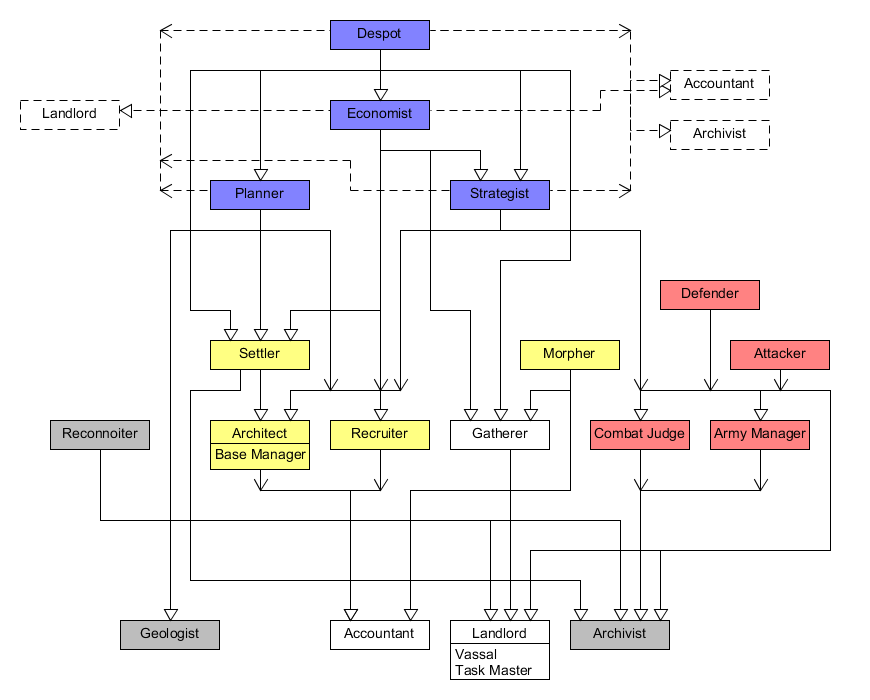
\includegraphics[width=\textwidth]{figures/Hierarchy}
\caption{Diagram of the module hierarchy}
\label{fig:hierarchy}
\end{figure}

%TODO Hierarchy diagram + description.

In the following chapters, we will describe the different groups of modules in the hierarchy and the problems they solve. While the modules are individually separate, some clusters of them are also separate. These can be separated in chapters as few of the modules has any connections between. The order of clusters is bottom-up so as to follow the chain of command. These groups are \emph{resources}, \emph{production}, \emph{information}, \emph{combat} and \emph{strategy}.

The following chapters cover the different groups of modules. They are:
\begin{itemize}
	\item Chapter \ref{ch:resources}
	\item Chapter \ref{ch:production}
	\item Chapter \ref{ch:exploration}
	\item Chapter \ref{ch:combat}
	\item Chapter \ref{ch:strategy}
\end{itemize}

Finally, Chapter \ref{ch:results} presents and discusses the results of the bot and the project as a whole.

	\subsection{Implementation}
	%Tidligt i rapporten, evt. som underafsnit til Agent Design. Her ville afsnittet primært handle meget overordnet kode-stil og om hvordan officer-systemet er implementeret:
	%- Er der brugt interfacet, templates eller andet finurligt?
	%- Hvordan snakker du med BWAPI? Problemer? Løsninger?
	%- Hvordan fungerer informations-udveksling mellem officererne?
	%- Hvordan fungerer kommando-mekanikker: direkte funktionskald, push "kommandoer" på en kø til senere inspektion, sæt et flag, osv?
	%- Var dine løsninger til ovenstående ad-hoc, løbende revurderet eller fra starten af grundigt og systematisk indtænkt?
		
	%Derudover kunne du have en kort beskrivelse af din generelle brug af C++
	%- C++11 eller ældre?
	%- Bruger du STL til data strukturer?
	%- Har du fulgt nogle særlige konventioner?
	%- Har du med vilje undgået visse subsets af C++? (dette er normalt fordi C++ er et lidt sygt sprog) Hvorfor?
	%- Er din kode systematisk kommenteret? Hvordan?
	%- Hvor mange kilde-filder har du og hvor mange linjer kode er der i alt?
	
		\subsubsection*{Programming API}
		\emph{BWAPI} is an API for StarCraft Broodwar and is injected upon startup by \emph{ChaosLauncher}. It loads an AI module written in c++, which can retrieve information about the current match's map status and send commands to the game through BWAPI. This controls the player's actions and allows the development of agents for StarCraft.
		
		Depending on the settings in BWAPI, the agent can be disallowed to retrieve information a player would not be able to. This means some units are in some levels of accessibility, where invisible and destroyed units are completely inaccessible. This has some limits however, as the agent can retrieve information about burrowed and cloaked units as if they were not. While a keen player can spot these units as they are not completely transparent, the agent has no limits as if they were completely visible, giving it an advantage. Additionally the agent is not limited to what is visible currently on the display, but can retrieve information from all over the map.
		
		There is a popular library, the \emph{Broodwar Terrain Analyzer} or \emph{BWTA} for short, which pre-processes maps for locations of interest. Most importantly, it marks the optimal depot locations for harvesting resources. While BWAPI already does this for start-locations, BWTA also does this for all resource clusters, marking viable expansion locations. The pre-processing of the map only has to be done once as the results are stored for subsequent games on the map. This library is automatically included in the 3.7.4 BWAPI test bot, so it is probable that almost all bots use the library.
		
		As an additional note, BWAPI divides the map into \emph{regions}. These contain satellite data about the borders to neighboring regions, included resources and base locations. They are important because the regions are separated in \emph{chokepoints}, which are either ramps or bottlenecked passages. Usually a region only contains a single base location and resource cluster, however some regions contain multiple clusters with overlapping base locations. Because of these qualities regions can be used to mark occupied locations by players.
		
		While newer versions of BWAPI exist, the 3.7.4 version is still widely used as it is considered the most stable, and is compatible with BWTA. There does exist a BWTA clone for 4th versions, however it is not very stable. The downside to 3.7.4 is that it does not support c++ 11. There does not exist an equivalent to BWAPI for StarCraft 2, since technically BWAPI is a hack and using it would result in a ban. AI's have been scripted in StarCraft 2's own editor however, and some have even gone and interpreted the display output of the game for a bot.
													%Chapter 2
%Contains base and resource management, specifically the TaskMaster.
\chapter{Workers and Resources}
This chapter covers the basics of gathering resources in StarCraft with a bot. 

In early- and mid-game, \emph{economic advantage} is the most important aspect of StarCraft strategy. This occurs when you have a higher resource intake than your opponent, such as if you have more workers that are gathering or more bases to gather from. The advantage is while maintaining an equivalent army to the opponent, one can replace lost troops faster, gain a larger army or upgrade the current one. If you eclipse your opponent in resources, you can perform worse in combat and still win. Without the advantage, upgrading troops would slow troop production down and the opponent could produce an equivalent or even stronger army at any time.

There are three kinds resources in StarCraft. \emph{Workers} are the only units capable of gathering resources. Each race has one worker type and each player start the game with a couple of their race's type. Players also start with a \emph{resource depot} or simply \emph{depot}. This structure can produce new workers and is also the drop off point for gathering resources. The Protoss worker is the \emph{probe} and their depot is the \emph{nexus}.

\emph{Minerals} are mined from mineral fields which usually are in clusters of 8-12. All units cost minerals, so it is the most important resource. Workers that mine these bring them back to the depot in batches of six mineral units. Depot's are limited in their proximity to the clusters, but at optimal distance there can be 3 workers on each field. Mineral fields are usually placed in a half-circle formation, such that there exists an optimal depot location. While the first worker on each mineral field will gather at a linear rate, they will yield diminishing returns on the second and especially third worker.

\emph{Vespene Gas} or simply \emph{gas} is harvested from \emph{refineries}. Each race has a distinct refinery structure, although they are very similar. These must be built upon \emph{Vespene Geysers} of which there are up to two by each mineral cluster. It is harvested in batches of eight with a max of three workers per refinery at optimal depot distance. Advanced structures, units and all technologies depend on gas. The immediate cost of the refinery and lost mineral gathering is a liability against fast openings, but harvesting too late means fighting against stronger units.

The last resource, \emph{supply} is a population limit and is not gathered like the other resources. Each unit reserves some amount of supply which is released upon their destruction. The only way to secure more supply is building the race's \emph{supply structure}. Each of these add some amount of supply to the total, which is subtracted if they are destroyed. Units cannot be produced if they require more supply than the player has free. If the player happens to reserve more supply than their total, they will be unable to build more units until more supply is acquired, called \emph{supply blocked}. Although supply is specifically the Terran resource, it is used as the general term for all races. \emph{Psi} and \emph{control} are the Protoss and Zerg equivalents. The Protoss supply structure is the \emph{pylon}.

While multiple workers can gather from the same field or refinery, only one worker can actively occupy it. The rest is either returning cargo, moving to the resource or waiting.

In the next sections we will first describe the architecture behind worker management, followed by how minerals is mined and gas is harvested. Building supply is first covered in chapter \ref{ch:strategy}, as this resources behaves much different than the others.

\section{Managing gathering}
%TODO Base Location description.

The \emph{TaskMaster} module contains workers at a single base location, and records their current tasks. It can return all workers with a specific task. Each base location is a wrapper \emph{Vassal}. The \emph{Landlord} module contains all vassals. None of these three modules have any agency, and only respond to function calls from superior modules.

%TODO Taskmaster implementation

Gatherer module accesses the Landlord module and with it, all the subordinate TaskMaster modules. Gatherering must be contained in a single superior module rather than within each Vassal, as gathering is not necessarily uniform across all bases.

\section{Mining Minerals}
StarCraft has a built-in worker gathering AI to help human players. Workers will automatically return cargo from resources (unless they are interrupted) and return to the same resource afterwards. When gathering minerals, they will move to another mineral field if the current one is occupied. This is an inefficient solution, as the worker could be stuck moving between minerals for long periods of time. It is also a liability for a bot, as the AI cannot be disabled. When harvesting gas they will wait until the refinery is unoccupied.

The simplest mineral gathering implementation is ordering idle gatherers to mine some arbitrary mineral. At some point, the built-in AI will ensure the workers are optimally scattered. It will however not be scattered immediately, and some workers will be very inefficient while moving from mineral to mineral. A simple but effective addition would be to scatter the initial workers.

By maintaining a queue of minerals, we can optimally scatter the workers. The first element of the queue is the mineral with fewest workers and the one in the back has the most. By continually assigning new workers to the first element and moving it to the back, we maintain a queue where the last mineral has at most one more worker than the first. Removing workers however requires finding the mineral in the queue, and should be done sparingly. Therefore, it is assumed any building or defending activity will be short and temporary, and workers assigned such will not be removed from the scattering. This might result in an ineffective scattering at some points. It is not clear however if optimizing the scattering at all times results in optimal resource output, as workers might be moved between minerals too often, resulting in less time mining.

If we maintain a dictionary of workers and their targets, we can assign new ones in constant time and retrieving targets in logarithmic time. This could be improved to amortized constant time with hashing. Removing a worker however requires a search through the queue which is linear time.

%TODO alternatives.

\section{Harvesting Gas}	
Gas harvest is very much like mineral mining, but simpler. Rarely will players have fewer than three workers on each refinery, as refineries will be built only when needed. Furthermore, almost all late-game units require gas, and harvesting is slower than mining.

The implementation is identical to mineral mining. No AI tournament maps contain more than one refinery, but the gas harvesting still uses a priority queue. In this case however, all operations become constant time, so performance is not harmed while code is reused.											%Chapter 3
\chapter{Production}
\label{ch:production}
This chapter concerns the creation of units including the architecture for its management. First we explain the StarCraft terms of units and their production.

A \emph{unit} is any player controlled entity, structure or not. Resources are also units, controlled by a neutral "player", but are both immobile and indestructible. Some spell effects, like the Terran nuke, are oddly also classified as units but they are neither selectable nor controllable. The term unit rarely includes these however.

\emph{Production} here refers to the player controlled act of creating a new unit. Within StarCraft, producing a structure is called \emph{building} and \emph{training} if it is a non-structure. Once a unit is created, there is a duration where it is \emph{constructing} before becoming \emph{complete}. A unit cannot execute player commands and has no abilities during construction. Constructing structure are placed in the world when they are built, while non-structure are hidden within their constructor. When a non-structure is complete, it appears at the nearest free space around its constructor. A unit consumes resources upon production, including supply requirements. A constructing non-structure can be canceled for a full refund.

BWAPI notifies the agent whenever a unit is created or completed in separate events, which can be used to update internal data-structures.

In the following sections we first briefly describe our location in the hierarchy. Then we begin with training of non-structure, moving on to building structures. Finally we cover expansions and expanding.

\section{Production Architecture}
The \emph{Accountant} module is used for keeping internal track of spent resources and scheduled units. Commanding a unit to build or train will not spend resources until at least the next frame. Therefore it is required to keep internal records of these, otherwise different modules might spend the same resources twice. Unit scheduling is useful in later frames, such that modules do not request the same unit multiple times.

Training is handled by the \emph{Recruiter} module, while building is done by the \emph{Architect}. These are separate modules as the two jobs are very different in implementation. While the Recruiter is quite low in the hierarchy, but the Architect is not since it requires workers from the Landlord module. Both are superior to the Accountant.

There is a third module, the \emph{Morpher}, which handles the rare case of a unit that executes a \emph{morph} command. A morphing unit transforms from one type to another, which is most often seen in case of building refineries. Counter-intuitively, the geyser morphs into a refinery and changes ownership to the constructing player, but the refinery is still built by a worker with a build command. The Morpher exclusively monitors morphing units, while the Architect handles the building.

\section{Training Units}
\label{sec:training}
The \emph{Recruiter} needs to be low in the hierarchy, as it needs to be accessed by many other modules. It does not contain an independent AI, acting only through certain events and method calls. The current implementation is generic such that it can handle any train-able unit in the game.

To train units, the steps are twofold: issue the train command to a relevant, available trainer and then monitor the construction.

	\subsection*{Commanding Trainer}
	Some units can train others, such as the depots that train workers. It is almost exclusively structures that can train. A unit can only train one at a time, although multiple can be queued up. Every unit is trained by at most one other unit, so a graph of trainers and trainees would be a \emph{forest} structure.
	
	Notice that it is inefficient to queue training, as this will lock resources. Instead, issuing the train command whenever the trainer is available will keep resources free without resorting to cancellation. It would be better to implement an internal queue if one was needed.
	
	To command the training we require the trainer. For this we would like to keep records of all units capable of training. BWAPI inherently contains the trainer of any given unit type, so using a dictionary of trainers with their types as keys is sufficient and allows fast queries. From this we can search through the set of trainers until we find one that is available and then send the train command. The evaluation of trainers involve verifying the current existence and control of the unit, and ensuring it is not currently training another unit or has been commanded to in this frame.
	
	Searching through the dictionary is logarithmic and iteration through the matching trainers is linear. Evaluating a trainer is constant. Given $n$ trainers and $m$ trainer matches, the time complexity for training is $\log(n) + m$, which could be improved to $m$ with hashing. Neither $n$ or $m$ are usually very large, but $m$ especially is only in the range of zero to four. Insertions and deletions of trainers are both logarithmic to their size.

	\subsection*{Monitoring Trainee}
	Other modules require to know which units are currently scheduled when planning their actions. Units could also be destroyed before completion, in which case other modules might need to reschedule.
	
	Once the train command has been issued, the Accountant is notified of the costs and the type.
	
	Upon receiving the event that a unit has been created, the Recruiter frees the resource costs from the Accountant, as the game state by now has withdrawn the costs itself. The Recruiter inserts the unit into a set of incomplete units. When a unit is completed, the Recruiter is notified and removes the unit from the set and from the Accountant. The same happens if the unit is destroyed, which occurs if the trainer was destroyed.
	
	Inserting and removing from the set is logarithmic to the size. The set is never expected to be very large.

\section{Building Structures}
Like training units, building structures is done in two steps: the structure is built and then it is constructed. Contrary to training, structures require both workers and a location to be built. Workers are the only units capable of building structures, and must move to the build location to do so. Terran workers must stay and construct structures until they are complete and Zerg workers are destroyed upon building, while Protoss require neither.

However, all Protoss structures must be in close proximity to a Pylon when built, and stops functioning without. The only structure exempt from is the depot and the pylon itself. This only becomes important in later stages of the game where Players might have to carefully manage their space. The agent is not expected to build enough structures for this to be an issue, so it is mostly disregarded. A Protoss structure is considered \emph{powered} when in vicinity of a pylon.

	\subsection*{Structure Placement}
	The Protoss player must place at least one pylon in any area he wishes to build in, and could distance pylons in a base to maximize coverage. Alternatively, if only a few pylons power a structure it creates a liability. The pylon could easily be destroyed to disable the structure, which is useful if it is a defensive structure or unit trainer. Fortunately, we expect the agent's bases to be compact enough such that we can place pylons somewhat arbitrarily and still manage to fit needed structures in the region. It is important however to place at least one pylon in a base before other structures can be built, but this is solved by the strategy modules.
	
	Unless a building location is specified, the easiest solution is placing a structure as close as possible to the base location in the desired region. All the workers in the region are usually at the mineral fields by the depot, and therefore will not be far from the placement. The workers and depot become sheltered by the structures, such that the opponents troops are forced to move through bottlenecks to get the workers. Even if a region only has one exit, it might be desirable to spread structures as flying units can attack from any angle. Finally, the solution is easily implemented.
	
	There are some exceptions. Depots will always be placed in new base locations and refineries can only be built on of vespene geysers. In both of these cases the building location will be specified by the superior module ordering the structure.

	The Architect attempts all locations in the map in a spiral pattern around the depot, and returns the first location that is available. This is simple, usually cheap but very expensive asymptotically, as it will be linear to the map size. However we never expect to visit anywhere near all the locations, since few tiles in the map cannot be built upon. To determine availability of a location, it must be clear of units and the tile terrain itself must be able to be built upon. Both of these are handled by BWAPI. Note that this solution places structures in a square pattern, which is not actually the closest to the base location except in \emph{taxicap geometry}.

	Placing structures too close can block passage between them, especially for larger units. The hitbox is arbitrarily different between otherwise equal sized structures in StarCraft, such that some combinations next to each other will block some units but not necessarily all. This is because the structure hitbox usually does not cover its location completely, allowing some leeway for smaller units.
	
	By placing structures at least one tile from each other, we ensure all units can easily pass through. This is done by keeping a map of all owned structure locations, where their dimensions are increased by one tile in all directions. If a build location overlaps any of the occupied tiles it is determined as not available. Registering new structures and querying this is constant time operations, but the space used is linear to the map size. It could be improved by only keeping a map for regions we have bases in, although not an asymptotic improvement.
	
	Additionally the Architect avoids placing structures between resources and depots to avoid obstructing workers. By drawing the smallest rectangle including the depot location, geyser(s) and mineral fields, the Architect avoids blocking workers by not placing structures within this. Building the rectangle is linear to the amount of items in it and querying it is constant, but we expect the amount of items to be low (ten or less). This structure map is handled by the \emph{Base Manager} module, which the Architect is superior of.
	
	To summarize, if a location is not specified, structures are placed in a spiral pattern around the depot, distanced by one tile from others and outside the gathering-zone.

	\subsection*{Aquiring Builder}
	Recall the Task Master module from Chapter \ref{ch:resources}. Since all workers are separated in base locations, we can easily pick a worker from the region the building location is. As the task master marks the jobs of all workers, we can pick a worker from either idle, mineral mining or gas harvesting (in that order). This way we do not interrupt other possibly important tasks. The Architect searches through the groups until it finds a worker that is not carrying resources, which then becomes the builder and is tasked as such in the Task Master.
	
	The time complexity is linear to the amount of workers in these groups. However, it is probable that less than half the workers are returning resources at any given moment, so it is expected that we only need to check two workers before finding a viable candidate. In case there are idle workers, the operation is constant.
	
	This solution does not work if we have no workers in the region. This is the case when expanding, where the worker must be specified by a superior module. This is the case when the \emph{Settler} module builds an expansion, explained in Section \ref{sec:expansions}.
	
	\subsection*{Executing Command}
	Once the builder has been retrieved, it will be commanded to build at the specified location. A player cannot build in hidden terrain, so the worker will first be moved closer to the target location in this case. When the entire placement has been revealed the builder is commanded to build the structure.
	
	The build order will then be stored in a set, containing the structure type, builder and location. Every frame, the Architect verifies the validity of the build orders, including verifying the builder has not been re-tasked. It also reissues commands to builders if required. As with monitoring trainees, incomplete structures are important to keep for the same reasons. In case of structures, there are more things that could go wrong which would incur cancellation of a scheduled structure. The builder might be destroyed or the build location might prove to be invalid upon being revealed.
	
	All invalid orders are removed, forcing superior modules to reissue the build order. This is desired compared to repairing the order, as the build order might no longer be required.
	
	\subsection*{Monitoring Constructions}
	Since Protoss structures auto-construct, the implementation is identical to monitoring trainees with the same time and space complexities.
	
	As mentioned prior however, refineries are handled by the Morpher module. BWAPI is notified when a unit morphs, upon which it is inserted in a set of incomplete morphs. A morphing unit is not considered constructing, although it is incomplete. When a unit is finished morphing, no event is called, therefore forcing the Morpher to verify all morphs every frame. However, there are very few expected morphing units at any given moment.

\section{Building Expansions}
\label{sec:buildExpansions}
Recall that \emph{expansions} are additional depots beyond the initial one, built at new resource clusters. As explained in the chapter \ref{ch:resources}, it is often profitable and sometimes necessary to expand resource harvesting to new locations. To avoid transporting cargo all the way between regions, players have to build depots near resources they wish to harvest.

When BWTA analyzes a map, it marks all viable depot locations. These are positions in which a depot will be at optimal distance from nearby minerals and geysers. Usually every resource cluster only has one of these positions, but some locations may contain overlapping depots. Regions rarely have more than one base location. Given a region, we can obtain all internal base locations, including these depot locations.

This significantly simplifies the construction of expansions, however the base location to settle must still be determined.

The \emph{Settler} module is responsible for all expansion behavior, and is also used to determine if expanding is possible. To build an expansion we need to specify a location and builder. These are handled by the Settler module, while the rest is done by the usual build procedure in the Architect.

	\subsection*{Expansion Placement}
	To determine whether a base location is fit to expand it must not already be expanded upon or contain enemy forces. Additionally, it must be reachable by non-flying units and have a path of regions without enemies. If these are satisfied, we consider the base location available for expansion.
	
	From the starting region, we visit neighbor regions recursively in order of proximity by using a priority queue, where the lowest priority is picked first. Initially the start region with priority 0 is inserted. When we visit a region, we visit all contained base locations. If any are available, we return one as the target location of expansion. In case none are available, but the region is unoccupied by enemy forces, we add all unvisited neighbors to the queue. The priority is equal to the distance between the two regions centers plus the current regions priority. If the region does have enemy units within, its neighbors are not added to the queue. The algorithm terminates when the queue is empty or an available candidate has been found.

	This solution satisfies our expansion requirements, and additionally includes the starting region should the depot be lost. It is very crudely implemented however, and quite expensive. Determining whether a region is occupied involves checking all enemy units. Given $r$ regions and $n$ enemy units, the time complexity is $rn$. This could be optimized by first marking all occupied regions before the recursion.
	
	The enemy units are retrieved from the \emph{Archivist} module, detailed in Chapter \ref{ch:exploration}.
	
	There could exists more factors when determining expansion locations beyond distance. Resource quantity or defensibility are also important, but are not considered here. One could favor regions distant to the opponent for added defense or alternatively closer for better map control.

	\subsection*{Expansion Builder}
	An expansion is often the first structure in a region, and therefore the player must acquire a builder elsewhere. The Architect only attempts to pick workers from the region the location is within, so the Settler must specify a worker beforehand.
	
	In this case, we just pick a free worker from the main base. There could be workers closer to the destination in other regions, and in this case the solution is sub-optimal. Recursively checking neighbors in order of proximity would result in an approximation of the closest worker. It was not a priority however as the improvement would be insignificant.
	
	The solution is cheap, and costs the usual to pick a worker. A worker considered available is either idle or tasked with gathering.										%Chapter 4
\chapter{Information Management}
One of the challenges in StarCraft is the imperfect information players have of the world. It is necessary to extrapolate the strategies of opponents from a few sightings, and regular scouting is mandatory. The player with the most perfect information can make the most optimal decisions.

In terms of bot development, there needs to be database systems for tracking information, and there needs to be a scouting AI.

\section{Tracking Units}
Initially, two things must be recorded for each enemy unit: position and type. The former is obviously needed to track movements of the enemy army to detect proximity of ones own army, and to record enemy base locations. The latter is needed as some units can change their type, such as the Protoss Archon. As an odd effect of the StarCraft engine, the Siege Tank changes types when it goes into or out of siege mode.

This was easily implemented with dictionaries with units as keys. Every frame, the bot updates all stored values. New unit are added based on events, as a newly revealed unit calls the \texttt{discover} and \texttt{show} events. The implementation uses logarithmic time on queries, additions and removals, but this could be improved to amortized constant time with hashing.

As a curious addition, geysers behave very oddly in the StarCraft engine. When a refinery is built upon a geyser, it actually transforms the geyser object. If the refinery is destroyed, a new geyser object is created. While all the initial geysers are known to players, new ones are not. This makes the tracking of geysers and refineries a bit difficult, as geysers must be checked every frame, and the new geysers must be detected.

The \texttt{Archivist} keeps track of all opponent movements. \texttt{Geologist} keeps track of current known geysers in the world.

\section{Scouting}
Scouting is important throughout the entire duration of the game. Early on, players need to know where the opponent is, what faction they are playing and which strategy they are employing. Later on, observing the enemy army size, unit types, base expansions and tech level is important to counter strategies.

The opponents faction is important when deciding on opening strategies. The factions behave very different early in the game. Openings are a decisively slower when one has to defend against every possible attack. Only if the opponent picked random as a faction will it be hidden. No units are shared across factions, so the first unit discovered will reveal it, which usually is their scout or main-base.

	\subsection*{Initial Scouting}
	The map terrain, along with resource locations, are completely revealed at match start. This includes all possible player start locations. Scouting for the opponent base is then just going through all other start locations. Maps used in competitive matches are usually no larger than four-player size, meaning there are four possible start locations. A player then has to take into account that they might have to scout up to two bases before knowing the enemy start location. Usually a player wants to know more than where the opponent starts, so even when it is deductible where the opponent is, the player wants to scout the base itself.
	
	Once the enemy base has been revealed, and with it his opening strategy, the scout is not useful any longer. It is a long trip back to gathering resources, and the scout might be followed, revealing your own location. Harassing enemy workers can put a dent in the enemy economy, even if none of them die. Simply by attacking enemy workers forces the opponent to pull two from gathering to defending. From there, the harassing scout can retreat until it is no longer chased, or lead chasing workers around while attacking passive gatherers. If the scout manages to kill a worker the opponent will fall behind in economy. However, compared to competitive human players, bots are usually too inefficient to take full advantage of this, but every bit helps.
	
	There are additional uses to the scout however compared to harassing. These must all be considered in the grand strategy, as they involve spending resources. These strategies include proxy bunker, photon cannon, barracks or gateway, manner pylons or gas stealing. Proxy structures involve building right below the enemy ramp or even inside their base. The usual distinction here is whether the structures keep the opponent in with defensive towers or rush attack with front line troop producers. Manner pylons are used in conjunction with these as Protoss, where the required pylon for forward bases are placed within the enemy mineral line, blocking and possibly caging enemy workers. Gas stealing involves building a refinery on the enemy geyser, blocking gas harvesting and forcing tier one unit use. While proxy troop production has not seen much use in bots, both gas steal and proxy towers has been used for varying effect.
	
		\subsubsection*{Implementation}
		Usually build orders include specifically when to send out a scout. In case of Protoss, the scout is often a worker that has just warped in a structure. This would however require a build-order system capable of containing other elements than builds. A simpler solution which is used here is sending a scout when a specific supply limit has been reached. This is noted in build orders, allowing for only slightly inaccurate build-order implementations.
		
		When picking a scout, the bot searches through different worker groups. First the idle, then the mineral miners and finally the gas harvesters. When it comes across a worker not currently carrying any resources, it assigns it as a scout, removing it from the \texttt{TaskMaster} in the mean time. Contrary to building or defending, scouts are assumed to not return, so it can safely be removed from the local worker pool and harvesting. If the scouting manager is unsuccessful in finding a worker, it retries next frame.
		
		While we have a scout and do not know the opponents position, we pick an unexplored base location and move the scout there. A tile is unexplored if it has never been revealed for the duration of the game. Thus, our home base will not be considered for scouting, and once the scout reaches the destination the tile will be explored, removing it from the possible scouting locations. Exploration is handled by BWAPI.
		
		This implementation scouts as long as no enemy buildings are known, extending its use into late game. Usually fast or cloaked units are used to scout later in the game, but it is not necessary.										%Chapter 5
\chapter{Combat}
\label{ch:combat}
This chapter explains how combat is handled in StarCraft, how its outcomes can be predicted and how the agent manages troops, attacking and defending.

Combat in StarCraft can easily become the most complex part of bot development. Multiple studies has been done on just small subsets of artificial combat scenarios, with specified units and simple terrain, but even these just scratch the surface of the field. Like the macroscopic strategies in StarCraft, there is likely no optimal command scheme for ones units. Predicting the outcome of a combat scenario, is therefore only done as approximations. This is also one of the areas where bots can excel against humans, since they can easily command different units in complex ways.

\emph{Troops} or \emph{fighters} here means units used for combat. Almost all non-building units beyond the workers are used in combat. Some units called \emph{spellcasters} deal damage indirectly through their abilities, while \emph{support} units help others fight better.

Every unit has some amount of \emph{health}, and almost all units can \emph{attack} to deal \emph{damage} to others. There are a number of additional factors such as armor and damage types, splash and hit probability, but it is sufficient to know that a unit loses health relative to the damage it is dealt. When a unit reaches 0 health, they are destroyed. Units attack at different ranges, such that \emph{melee} units need to be close and \emph{ranged} units can attack at a distance.

In the following sections we will explain the base management of troops. Then we move on to combat prediction, followed by attacking and defending.

\section{Managing Troops}
The \emph{Army Manager} is the troop parallel to the Task Master from Chapter \ref{ch:resources}. It contains all fighter units controlled by the agent and their current assigned \emph{duty}, same as the \emph{tasks} for workers from Section \ref{sec:manageWorkers}. The current types of duty are \texttt{idle}, \texttt{defend}, \texttt{attackTransit} and \texttt{attackFight}. Distinct from the Task Master, there is only one instance of the Army Manager, as troops are not separated into regions.

\section{Combat Prediction}
Predicting the victor of combat is very difficult in StarCraft and predicting the specific casualties is neigh impossible. Even beyond the numerous factors in combat, the optimal command of troops is completely Dependant on the opponent's commands. Unless the opponent operates in a recognizable pattern, they movement is unpredictable. Predicting combat is therefore more based on what units the opponent controls, how the terrain is and then either a theoretical upper limit of their damage output versus a prediction of our own.

Some of the most successful predictors simulates a simple form of combat and evaluates the result. This however assumes how the opponent will control its troops, or at least assumes it knows the optimal control scheme. Neither of these are possible, especially not with incomplete map information, but the results are usually close enough. SparCraft uses this method with good results, but even it ignores multiple factors including collision.

The combat prediction algorithm resides in the \emph{Combat Judge} module, which is used only by the Attacker and Defender, covered in this chapter, and the \emph{Strategist} covered in Chapter \ref{ch:strategy}. Given a set of units, it returns a value representing the \emph{strength} of them. The army with the higher value is predicted to win in a confrontation.

Following is a description of the prediction heuristic: let us assume a simple scenario: two units, $a$ and $b$ are attacking each other. We have the health values $h_a, h_b$ and the \emph{damage-per-second} (DPS) values $dps_a, dps_b$. Assuming both units start attacking each other at the same time, then we must have $TTK_a = h_b / dps_a, TTK_b = h_a / dps_b$, where $TTK_a$ and $TTK_b$ are each unit's \emph{time-to-kill} (TTK). This value represents the time in seconds it takes to kill the opponent. It must be the case that the unit with the lowest TTK becomes the victor, and with this we can predict the outcome of the simple situation.

Notice that we can simplify the solution and instead simply compare the values $s_a = h_a dps_a$ and $s_b = h_b dps_b$. This enables us to value the strength of an unit independently of the enemy, which is quite helpful when pulling workers one at a time in Section \ref{sec:defending}.

We would like to scale the solution to armies by using the sum of strengths as the army's strength. This requires the additional assumption that no units are destroyed during combat. If this happened the TTK would not be constant, changing the outcome. This is almost never the case in real combat scenarios, and can cause the prediction to be inaccurate. This happens when armies have the same strength value, but not the same amount of troops, where the largest army is overestimated.

The prediction was already inaccurate however, as we never take terrain or range into account. For this reason, the prediction underestimates Terran units, which are all ranged. Additionally the prediction has two properties that are not true. Firstly the strength of armies increases linearly with its size, which is not necessarily true in-game. When grouped, the units destroyed last will have dealt more damage than possible if attacking one at a time. Secondly the comparison between armies is non-transitive. The units in StarCraft (and most RTS games) are designed like a rock-paper-scissor game, such that army $A$ beats $B$ and loses to $C$ while $B$ beats $C$. This means the strength of an army is relative, and cannot be accurately evaluated as an absolute value like here. 

However, this solution has proven to be sufficient in the early game. Protoss has the strongest early unit, which mitigates the disadvantage of attacking when outnumbered. The units will usually be able to destroy one or more of the enemies, such that both players loses troops. The only case where this is not true is against other Protoss players, but here the prediction is perfect as both use the same early unit type.

The prediction is very cheap, having a time complexity linear to the size of the army and uses constant amount of space.

\section{Attacking}
\label{sec:attacking}
A player will almost certainly expand to their natural expansion first and expanding to a third base is only viable beyond early game. The natural expansion is very close to the main base and is usually right outside the only exit of the main base. This proximity allows us to consider both bases as a single base. From these assumptions we can conclude the opponent will only have one base for the duration of the early game, which is the only stage we are concerned with.

In euclidean space the shortest path between two points is the same regardless of which is the origin. In terms of StarCraft, the shortest path between the opponent's and the agent's base is the same regardless of which the troops move from. Assuming each player only has one base and both players will use optimal pathfinders, we can model the map as a straight line between the bases. Both armies will only travel along the shortest path and there is therefore no case of armies moving past each other without colliding.

When rushing, it is favorable to move troops as close to the opponent's base as possible without confrontation, even before they are ready to attack. This pressures the opponent, scouts the map, attacks the earliest possible time and distances the opponent's troops far from the player's base. Even if the fight ends in defeat, the opponent's troops will have to move across the map to attack, and in case of victory, the player's troops can continue towards the opponent's base with minimum delay.

When the we predict a victory in combat against the opponent army, we attack. In some cases it might be prudent to wait until more units have been amassed, especially if we produce more troops than the opponent, as we will sustain fewer losses and be more certain of a victory. This is difficult to asses while also being very risky, so the safer option is just attacking immediately.

Attacking is handled solely by the \emph{Attacker} module.

	\subsection*{Targeting}
	Most real-time strategy games has the unit command \emph{attack-move}, and StarCraft is no exception. A unit executing this will move towards a unit or location, but will attack any enemies along the way. The unit will prioritize attacking those that are damaging it. This command therefore auto-targets nearby enemies and also has simple, inherent prioritized targeting.
	
	By targeting the enemy base location or structures with this command, troops will automatically fight the first enemy they meet, which is either the opponent's base or army. The most important targets are the enemy structures, since destroying all of them is the win condition. The Archivist from Chapter \ref{ch:exploration} records all known enemy buildings, from which the Attacker picks one arbitrarily. With the assumption that the opponent only has one base, the army will attack the foremost building regardless of target, since they are attack-moving. In case there are defensive structures, the attack-move command will automatically re-target to them once they damage the army.
	
	This allows for constant time targeting retrieval. Alternatively some units could be prioritized, such as the enemy workers or troop producers, but this is otherwise the cheapest solution while still a good approximation of optimality.
	
	Some bots manually prioritize during combat. There have been studies on using different priorities, such as attacking the unit with highest health to resource cost ratio. This is a greedy attempt at costing the opponent as much as possible. A similar one is attacking units with highest health to damage ratio, or simply the unit with lowest health. There are more advanced strategies however when considering large scale armies composed of different unit types, where counter-play between individual types are important. The usual order of targeting is the opponent's army, then economy and then unit producers.
	
	\subsection*{Troop Rendezvous}
	Once any fighter unit has been completed, they are set to the duty \texttt{idle}. Every frame the Attacker will re-task all the \texttt{idle} troops to \texttt{attackTransit}. These units are commanded to move towards the enemy base, but not attack. Otherwise, they would attack the enemy base one at a time. Grouping troops is more efficient as the total health pool is larger, allowing the troops to deal more damage before they are destroyed. This has the opposite effect on the opponent's army, which has less time to deal damage. Therefore, it is more efficient to wait until more troops have arrived.
		
	At some point the troops will be within some distance of enemy units where they will risk being attacked. This distance is a bit larger than the longest range of any unit. Once troops are within this distance, the Attacker will use them for combat prediction. By only counting these arrived troops, the module can tell when there are enough to beat the opponent. If they are strong enough, the Attacker will re-task them to \texttt{attackFight} duty. In this state, they are commanded to attack move the target found prior. It is important to attack immediately when possible, as waiting too long will allow the opponent to counter the attack with stronger units or defenses.
	
	In case the \texttt{attackTransit} units within this danger distance is not strong enough, they will instead retreat towards the main depot. The result is troops moving back and forth right outside of enemy range, until enough troops have gathered. In case the opponent advances with a stronger army, the troops will retreat until outside their range. In case the enemy army reaches the base, the Defender module takes over the troops, which is explained in Section \ref{sec:defending}.
	
	\texttt{attackFight} units never retreat, fighting to the death. This is because it is difficult to determine when retreating is efficient. While troops retreat, the enemy army has the opportunity to attack them without receiving any damage themselves. In some cases retreating might be impossible if ones units are too slow. In case the army would sustain heavy losses, it might have been a better choice to destroy as many of the enemy troops as possible. All troops with the \texttt{attackFight} duty outside of enemy range reverts to the \texttt{attackTransit} duty, moving towards the enemy base once again.
	
	The Attacker only counts units currently within this danger distance of an enemy unit as arrived, that is, it does not record arrivals between frames. Testing proved the battlefield shifted too much to record arrivals and stopping troops until they were ready, as it lead them to becoming scattered across the battlefield sometimes. By only relying on the current situation, it is certain that the units are actually gathered.
	
	This current implementation is expensive as every unit compares itself with every known enemy to detect whether they are within range. Given $n$ troops and $m$ enemies, the time complexity is a polynomial $nm$ number of operations. All the remaining operations are asymptotically less than this however, so this is also the total. 
	
	There is not always enough space for all units to wait if the army is large, but it is usually not. A better solution would be needed however if the army was larger or contained large units. In this case, heat maps or cluster detection could be used to detect the density of the army.
	
\section{Defending}
\label{sec:defending}
If a player's base is under attack, different behavior is required compared to attacking. Even if outnumbered, it is favorable to fight the invaders. In case the defending player has no troops left, the workers function as a last line of defense. Usually the opponent will attack the workers first in any case, so they might as well fight back.

Since Protoss are quite slow, it is possible the opponent rushes first. In some cases, no troops might have been built yet, and it is up to the workers to defend the base. Zerg is very quick to produce troops and is capable of this, but other races could send workers to build a forward base. The usual case however is defending against the opponent's scout. Even if the scout simply stays in the base without attacking, it is important to destroy it quickly to starve the opponent of information.

Some strategies involve building static defense structures, which are stronger and cheaper than the mobile troops. These can be built very early if the player is determined, at the cost of expanding economy and not pressuring the opponent. Beyond early game, these defensive structures are usually always built to prevent ambushes and detect cloaked units. Rushing players however, favors mobile troops over these defenses.

The \emph{Defender} module is capable of defending with nearby troops, including workers if necessary, against any non-flying, non-cloaked threats. The module is a sibling to the Attacker in the hierarchy, but has a higher priority as defending the base is more important than attacking. Therefore the Defender is updated before the Attacker in each frame.

	\subsection*{Scrambling Defenders}
	The problem with acquiring defenders is related to the retreating problem. It must be avoided pulling troops back that would be better used attacking. Defending is an attempt at damage control, however the opponent must still be pressured with attacks as quick as possible. Some units might be too far away to participate significantly in the defense, in which case it should instead attack the opponent. In case both players are invading each others' bases, it becomes a race. In these situations, it is not always clear what the correct move is.
	
	In line with the non-retreating paradigm from Section \ref{sec:attacking}, we will assume that units already in combat should not be interrupted. Additionally, units within regions with expansions should defend, as the unit will be within reasonable traveling distance and is not currently attacking. Since the macro strategy is rush, units that are not within an region with expansions should continue to attack.
	
	As it turns out from testing and because of the single path model, the agent very rarely have any units left outside its base if the opponent is currently invading, as all prior units would already have fought and been destroyed. In case there are units beyond, they will usually have reached the opponent's base before his army invaded, in which case the correct decision is continuing the assault. The current solution has therefore proved to be sufficient.
	
	There is a slight issue because of the region clause. If the opponent has a large army which has not completely crossed into the defended region, the defenders will revert into attacking behavior upon destroying all those within the region. Sometimes the defending units will continually retreat and attack as parts of the enemy army moves into the region, sustaining more damage than is necessary. It is a difficult problem to solve however, as the Defender would need to detect and target the clusters of units rather than the individuals.

	Once all defenders have been assigned, they are commanded to attack-move an arbitrary invader. The defending units will then prioritize the closest invaders. If the invaders are defeated, all the remaining defenders will be set as \texttt{idle} in the Army Manager.

	\subsection*{Rallying Militia}
	Sometimes there are not enough troops in the base to defend. In this case, a common strategy is moving all the workers to defend.
	
	Once all available defenders have been assigned, the Combat Judge will calculate the values of the invaders and defenders. Until there are no more free workers or the defenders are stronger than the invaders, the Defender will task additional workers to defend. They are commanded in the same fashion as the rest of the defenders. Once the fight is over, all the defending workers will be re-tasked as \texttt{idle} in the Task Master.

	Alternatively, in case there are enough troops to defend, players might temporarily relocate workers to safe resource clusters until the conflict is resolved. This is rarely an issue in the early game however, and has not been a priority yet.											%Chapter 6
\chapter{Strategy}
\label{ch:strategy}
This chapter concerns itself with how we implement the overall strategic reasoning in our bot. We have already gone through the basics of strategies in StarCraft, and all the basic functionalities has been implemented in the bot. Now it must all be put together in a cohesive form to achieve a strong AI.

Initially the bot functioned purely on a greedy principle. Concerning a specific set of units, we attempt to produce them if possible every frame. This is possibly the fastest and simplest AI to implement, but it has proven to be an effective approximation in some algorithmic fields. As the bot was developed additional systems was implemented, but the core auto-pilot remained greedy.

The overall strategy of the bot is rushing. It needs to be effective in economy early on and build troops as fast as possible. It sacrifices long term advantages for an early game attack. If the initial attacks are successful, the bot would gain even stronger long term advantages by hindering the opponent, and would be able to transcend into mid-game tactics.

While one could focus on a niche strategy such as proxies or such, as explained earlier these strategies are strongly countered by some specific strategies. They are high-risk, high-reward, but only work in  a small subset of match-ups. So even though they would be effective in these match-ups, we would need to implement other solutions for the rest, where a not insignificant amount of them would require an advanced bot beyond these 'cheese' strategies. Therefore, we could just as well implement an advanced bot and cover all match-ups. All-in would be such a niche-strategy against humans, but bots have proved to be very ineffective against this strategy. Additionally, the all-in strategy is a more aggressive version of rushing, so it could easily be transformed into the latter without any large scale implementations.

All combat decisions are made by the \texttt{Strategist} manager, while economy decisions are made by the \texttt{Economist} manager. These are disabled by the \texttt{Despot} manager when executing a build-order. The \texttt{Despot} module is the highest in the hierarchy, beyond the core AI module receiving call-backs from StarCraft.

\section{Economy}
TODO intro

The \texttt{Economist} manager moderates worker production and expansions, unless it has been disabled by the \texttt{Despot}.

	\subsection*{Workers}
	Generally it is advised that a Protoss player keeps producing workers constantly until late-game, but some openings might temporarily stop worker production. Therefore, if we are not at the desired worker amount in a base, we attempt to produce a new worker with regards to resources and whether a worker is already in production.

	%Moved from Resources.
	%Usually a Protoss player should not stop building workers until late game, but some openings require a temporary pause in their production. Therefore the solution is just greedily building workers while no build order is being executed. 
	
	%Moved from resources.
	%\section{Building Supply}
	%A player can have a maximum of 200 supply. The simplest supply implementation is to build supply units whenever the supply limit has been reached while it is below the maximum threshold. This will however throttle production while the supply structure is being constructed, which is inefficient. The optimal solution would be predicting supply needed in the near future and interlace supply production with unit production such that all orders are completed the earliest. Observe however that this is alike the \emph{Job shop scheduling} problem but more complex with the additional factor of resources. As such the problem is NP-complete, and even then resource gathering rates must be predicted for optimal solutions.
	
	%Moved from resources.
	%A simple solution which is implemented in the current bot is to build supply units when released supply is below a set threshold. This threshold is somewhat arbitrarily set according to testing. A more dynamic solution would be to set the threshold to the amount of supply used if all production facilities built a unit, assuming the unit type can be predicted. This solution will build supply units that are completed before they are needed, but might not result the optimal amount of units completed at any given time (impacting economy with relation to workers). The worst problem, production throttling, is avoided however.
	
	%Moved from resources.
	%Maynard Slide
	
	%Moved from resources.
	%TBD Mineral to gas ratio.
	
	\subsection*{Expanding}
	An expansion secures a more permanent economic advantage, as a player secures both more resources and gathers them faster. More expansions also secures map-control, as the player will have more presence in the map and control more resources.
	
	Deciding when to expand is both difficult and pivotal. It takes time and resources and leaves the new base pretty vulnerable unless there is a standing army. A player with a stronger army can safely expand while guarding it, securing his advantage or at least keeping up with the opponents expansions. Without the stronger army its a risky maneuver, but might still be viable or even imperative. At some point the resources in ones current bases will be depleted, leading to a need to expand. If a player expands before having saturated his current mineral fields, its called a \emph{fast expand}, sometimes used as an opening. This is very risky but with a very immediate payoff in economy. The contrary formula, keeping a single base until mid-game or alike is called \emph{one base play}.
	
		\subsubsection*{Implementation}
		It is only clear that an expansion is viable when all mineral fields have been saturated. Before this, it is both risky as we sacrifice current resources for later economy, which requires both a strategic reason and foresight whether it is viable. By expanding when we have saturated our mineral fields, we risk expanding too late, but ensure a consistent worker production throughout the game. Expanding too late is better than expanding too early; an early expansion will waste resources or possibly result in an immediate loss, where a late expansion simply wastes an opportunity.
		
		Since expanding is a costly affair, the bot needs to save up resources. Therefore, the expansion is queued in the build-order, thereby pausing other productions until the expansion is ready.
		
		TBD Implement better expanding, avoid opponent regions and avoid if in combat.
	
		The bot can perform a fast expand opening, but it has not been very successful compared to its usual one base play. The difficulty lies in detecting whether a fast expand is viable, which is very much Dependant on enemy openings. It was decided to focus on the safer opening instead as it is a more versatile strategy.
		
		TBD Evaluation of the auto-expander vs. one-base bot.
		
\section{Combat}
TODO Combat intro.

Building troops.

Counter Strategies.

\texttt{Strategist} order the production of troops and troop facilities.

	\subsection*{Troops}
	As this bot is very simple in terms of handling units, it is appropriate to use the first available units and attack as quickly as possible. The idea behind this strategy is, that since this bot lacks greater strategic reasoning and handles late game units poorly, then it should attempt to win the game before any of that becomes relevant. This can beat more complex bots, simply because their otherwise superior strategies are never allowed to hatch. Additionally, Protoss has the strongest and easiest to use early game units, and when massed will easily beat both Terran and Zerg.

	Currently the bot just mass produces zealots whenever it can in greedy fashion. As producing zealots is the ultimate goal of the bot, this is sufficient.

	TBD Additions: Dragoons, upgrades.
	
	\subsection*{Facilities}
	It was found through testing that a single saturated start base can handle around four gateways constantly producing zealots. This gets more difficult to asses with expansions, and it was unfortunately also found through testing that greedily building limitless gateways is not even close to optimal.
	
	The current limited solution is building seven gateways at max. Usually if the bot reaches a point where it needs more, it has probably already lost due to lacking in technology. A scalable solution has not been implemented, but to be optimal it would require some estimation of resource input, along with estimated need for profit for further development of base and technology.

\section{Build-orders}
Openings in StarCraft are usually detailed like a \emph{build-order}, which is very much like a chess opening. Because of the huge decision space, even humans need some guidelines weathered by experience to perform well in the beginning of the game. The optimal build-orders have changed a lot across the years, shaping the meta-game of StarCraft. As new strategies were found, new openings had to accommodate new possible opponent strategies.

A build-order is a list of units that must be produced in a specific order, sometimes after certain events. There is no timer in vanilla StarCraft and using one is considered cheating in tournaments, so items in the build-order are to be constructed when specific supply costs has been reached. Between each item in the build-order, the player must produce workers until then next supply limit has been reached unless specifically otherwise instructed. 

This is akin to executing a queue of orders. One could make a queue where the next item is executed if a specific supply is reached while automatically building workers like a human player. The easier solution for bot however is of course manually filling in the gaps with worker orders, such that the supply limits will be reached at the correct times (assuming no workers are lost). Therefore, the solution in the bot is simply having a queue of units. While the queue is not empty, we do not execute any higher-order manager AI that would otherwise automate production. When the queue becomes empty, we resume automatic production.

The benefit of this solution is the ease of adding new openings to the bot. Although the general autopilot AI is the same, different openings will vastly change the strategy and outcome of the game. Proper openings are key to winning in early game, or at least not lose during. The downside however is the rigid planning structure, which can't allow for easy adaptations or responses. What if the bot loses a worker or a structure? It is possible that the current build-order is no longer optimal, viable even. We avoid this, by making sure the build orders are short, such that the opponent could in no way interrupt with any units other than harassing workers.

Additionally, this solution could be used to pause other production in mid-game. Since the bot operates in a greedy fashion, it can be difficult to build high-cost units. The solution is to enqueue the unit, pausing all other production until the unit has been created. This is used in the agent when expanding, where the depot is queued. This solution is risky however, as the bot will not consider removing the depot from the queue under any circumstance. It does not seem to cause any problems however, as the bot will reach the amount of resources required very quickly, resuming normal production again.

Since the build-order is a queue, executing it is constant time, and enqueuing the build-order is linear. The build-order is never changed during gameplay.

The \texttt{Planner} module handles executing build-orders. The main module \texttt{Despot} handles queuing build-orders and disables other managers while \texttt{Planner} is executing a build-order.											%Chapter 7
\chapter{Results and Evaluation}
\label{ch:results}
The bot was submitted to the SSCAIT. While the tournament itself has not started yet, the bots still play against each other in live-streamed matches. There is a scoreboard where bots are placed accodingly to their win-rate, with total wins and losses marked. As mentioned in Section \ref{sec:expanding} there are three versions of the bot, all of which has been submitted. The versions are "One-Base", "Always-Expand" and "Condition-Expand". The first version never expands, the second expands whenever desirable. The third behaves like the first version, until the opponent builds defensive structures where it switches to the second. Table \ref{tab:results} contains the results of the three versions.

\begin{table}
\begin{center}
\begin{tabularx}{\linewidth}{|X||l|l|l|}
	\hline
	Version				& Games	& Wins	& Win-rate	\\
	\hline
	One-Base			& $780$	& $527$	& $79.23\%$	\\
	Always-Expand		& $104$	& $78$	& $75.00\%$	\\
	Condition-Expand	& $79$	& $63$	& $79.75\%$	\\
	\hline
\end{tabularx}
\end{center}
\caption{Sparring results from the SSCAIT website}
\label{tab:results}
\end{table}

The initial One-Base version did very well, netting almost an $80\%$ win-rate. The next version, Always-Expand, was not tested as thoroughly, but it is clear that it did not perform as good. It turned out that by far most of the bots were aggressive rushers, which often would destroy the first expansion. At that point the bot would be behind in troops and quickly lose. This spurred the Condition-Expand version, where it would not expand against rushers. Unfortunately, it only marginally improved the win-rate, and with few enough games for the results not to be conclusive. This is probably because the expansions was not enough to win against the defensive bots, in which case the outcomes of games were unchanged.

As one could expect, the bot does well against others using boom-strategies and proxy-strategies. It wins by far most of the matches against other rush bots, including mirror-matches, except UAlberta bot as mentioned. It fares poorly against the turtling Terran bots, which quickly goes for more advanced units. The expansions were an attempt to combat the turtle strategy, but it was not enough. While the bot does gain an economic advantage, it never uses it to train stronger units.

SSCAIT accepts bots from non-students which only play in mixed-division where student bots play both that and the student-division. The statistics above is from the mixed-division, and there is unfortunately not a student-division only statistic. The One-Base and Condition-Expand versions are usually among the top 8 mixed-division bots and contender with a few for the first place in student-division. This is difficult to ascertain without clear statistics and will first be determined with the tournament results.

The bot will be entered in the 2015 AIIDE and CIG competitions, and further development on the bot is planned.

	\subsection*{Performance}
	Performance wise, the final version(s) of the bot do very well. SSCAIT monitors the frames as there are time limits bots must satisfy to upkeep the real-time aspect of the game. The rules are:
	\begin{itemize}
		\item no more than 1 frame longer than 10 seconds,
		\item no more than 10 frames longer than 1 second and
		\item no more than 320 frames longer than 55 milliseconds.
	\end{itemize}
	The bot has never lost a match due to breaking the time limits. In fact, it has not been observed to once exceed 55 milliseconds in a frame. Not unexpected however, since the bot has favored simple and very cheap solutions. There are certainly some algorithms that could be improved, such as detecting troops' proximity to the enemy. These are the minority however, and the current implementation allows for further development without reworking it.

	\subsection*{Features}
	The bot never reached any high-level, complex AI solutions. The focus was creating a competitive bot, so development focused on areas that improved performance the best. This turned out to be low-level technical features such as managing and commanding units and internal production data-structures. It was much more important that the bot acted correctly than it acted optimally, so simple solutions was sufficient in almost all aspects. Further development should focus on improving combat predictions and map awareness with regards to enemy unit placement, such that the bot can play in later stages of the match. Additional features would be controlling more kinds of units and better adaption to opponents' strategies.
	
	As the results show, the expansions did not improve performance noticeably. The economic advantage gained from expansions were not enough to offset the disadvantage of only using the earliest Protoss combat unit. By increasing the array of units used by the bot, the advantage of expansions may be clearer. In any case, expansions were needed at some point in the bot's development, as they are mandatory in longer games. In hindsight, it might have improved gameplay performance more if other features were pursued instead, like combat prediction or advanced units.											%Chapter 8
\chapter{Conclusion}
The bot has been a success with a $79.23\%$ win-rate as Protoss in mixed-division on SSCAIT. It handles basic StarCraft maneuvers such as harvesting both types of resources on multiple bases, building structures and executing a simple rush strategy. It can execute build-orders, including early expansions. When in combat, it can do basic tactical decisions such as gathering troops and retreating. With a very simple but somewhat effective combat prediction heuristic, it will attack only when ready. The project has achieved its goals of developing a competitive bot for StarCraft. While the bot is simple compared to humans and older bots, it is still above in complexity and effectiveness than the average.

The bot will be submitted to the 2015 AIIDE, CIG and SCAIIT competitions and further development is planned at least until the competition deadlines.

%Experiences										%Chapter 9
%\appendix
%\chapter{Stuff}

This appendix is full of stuff ...											%Appendix A
%-----------
% Backmatter
%-----------
\backmatter
\chaptermark{Bibliography}
\renewcommand{\sectionmark}[1]{\markright{#1}}
\sectionmark{Bibliography}
\addcontentsline{toc}{chapter}{Bibliography}				%Force addition of Bibliography to TOC
\bibliographystyle{alpha}									%Use alpha codes for references
\bibliography{References}									%Bibliography file called
\end{document}
% % % EOF % % %